\documentclass[a4paper,twoside,12pt]{article}
\usepackage[top=1.5cm,left=1.5cm,right=1.5cm,bottom=2cm]{geometry}

\usepackage[utf8]{inputenc}
\usepackage[T1]{fontenc}
\usepackage{lmodern}
\usepackage[brazilian]{babel}

\usepackage{graphicx}
\usepackage{subfig}
\usepackage{psfrag}
\usepackage{cite}
\usepackage[cmex10]{amsmath}
\usepackage{amssymb}
\usepackage{upgreek}
\usepackage{microtype}
\usepackage{titling}
\usepackage{courier}
\usepackage{url}
\usepackage{hyperref}
\hypersetup{
	colorlinks=true,
	linkcolor=blue,
	urlcolor=blue
}

\usepackage{tcolorbox}


\usepackage{booktabs}

\usepackage{calc}


% Use the 'listings' package to add code and the 'color' package to generate the highlights
\usepackage{listings}
\usepackage{color}
\definecolor{grey}{rgb}{0.6,0.6,0.6}
\definecolor{codegreen}{rgb}{0,0.6,0}
\definecolor{codegray}{rgb}{0.5,0.5,0.5}
\definecolor{codepurple}{rgb}{0.58,0,0.82}
\definecolor{backcolour}{rgb}{0.95,0.95,0.92}
\lstset{language=Python,				% set it to Python language highlighting
	backgroundcolor=\color{backcolour},
	commentstyle=\color{codegreen},
	keywordstyle=\color{magenta},
	numberstyle=\tiny\color{codegray},
	stringstyle=\color{codepurple},
	basicstyle=\ttfamily\small,		% set size of fonts
	breaklines=true,				% set automatic line breaking
	linewidth=\textwidth,			% set size of code box
	showstringspaces=false}			% show spaces as underscores only inside strings


\tcbuselibrary{skins, breakable}

\newtcolorbox{exercisebox}[2][]{
	colback=blue!5!white,
	colframe=blue!50!black,
	fonttitle=\bfseries,
	title={Exercício #2},
	#1
}

\newtcolorbox{theorybox}[1][]{
	colback=gray!8!white,
	colframe=gray!50!black,
	fonttitle=\bfseries,
	title={Conceito Teórico},
	#1
}

\newtcolorbox{notebox}[1][]{
	colback=orange!8!white,
	colframe=orange!60!black,
	fonttitle=\bfseries,
	title={Observação},
	#1
}


\title{\vspace{-2cm} Processamento Digital de Sinais e Aplicações em Acústica\\ Tutorial 08 - Janelamento e \emph{Zero-Padding}}
\author{\url{https://github.com/fchirono/Aulas_PDS_Acustica}}

\begin{document}
	\date{}
	\maketitle
	
	\section*{Objetivos do Tutorial}
	Ao final desta sessão, você será capaz de:
	\begin{itemize}
		\item aplicar uma função de janelamento na análise de vetores finitos com a DFT,
		\item entender as implicações na escolha de diferentes funções de janelamento,
		\item aplicar o preenchimento com zeros (\emph{zero-padding}) na análise de vetores finitos com a DFT,
		\item entender em quais condições causam o problema de \emph{vazamento espectral}, e quais técnicas podem ser usadas para mitiga-lo.
	\end{itemize}
	
	\begingroup
	\let\clearpage\relax
	\tableofcontents
	\endgroup
	
	
	% -----------------------------------------------------------------------
	\section{Introdução}
	
	A Transformada de Fourier Discreta (DFT) é uma ferramenta fundamental na análise espectral de sinais discretos. Contudo, sua aplicação prática sobre registros finitos de dados introduz o \textbf{vazamento espectral} (\textit{spectral leakage}). Este tutorial aborda as técnicas de \textbf{janelamento} e de \textbf{preenchimento com zeros} (\textit{zero-padding}), que mitigam ou caracterizam esses efeitos.
	
	% -----------------------------------------------------------------------
	\section{Fundamentos Teóricos}
	
	\subsection{A DFT e a Hipótese de Periodicidade}
	
	A DFT de um vetor $x[n]$, onde $n = 0, 1, \ldots, N-1$ são as amostras no domínio do tempo discreto, é definida como
	
	\begin{equation}
		X[k] = \sum_{n=0}^{N-1} x[n]\, e^{-j2\pi kn/N}, \quad k = 0, 1, \ldots, N-1.
		\label{eq:dft}
	\end{equation}
	
	As frequências discretas $k$ correspondem às frequências analógicas (em Hertz)
	
	\begin{equation}
		f_k = k \, \frac{f_s}{N} = k \, \Delta f,
		\label{eq:freq_resolucao}
	\end{equation}
	
	\noindent onde $f_s$ é a frequência de amostragem em Hertz e $\Delta f = f_s / N$ é o intervalo entre duas frequências discretas.\footnote{O valor $\Delta f = f_s / N$ é coloquialmente chamado de \emph{resolução em frequência} - porém, a definição correta de resolução em frequência descreve a capacidade de distinguir duas frequências próximas, conforme veremos a seguir.}
	
	Um ponto fundamental é que a DFT pressupõe implicitamente que a janela de $N$ amostras representa \emph{um período} de um sinal periódico. Ao computar a DFT, assume-se que o sinal se repete indefinidamente tanto para $n < 0$ quanto para $n \geq N$. Quando essa hipótese não é satisfeita — isto é, quando a janela de observação não contém um número inteiro de períodos —, surgem descontinuidades nas junções entre repetições periódicas, dando origem ao \textbf{vazamento espectral}.
	
	\subsection{Vazamento Espectral}
	
	Considere um sinal cossenoidal de frequência $f_0$, período $T_0 = 1/f_0$, e amplitude $A$:
	
	\begin{equation}
		x(t) = A \cos(2\pi f_0 t).
		\label{eq:cosseno}
	\end{equation}
	
	Se o vetor tem duração $T = M \cdot T_0$ (com $M$ inteiro), exatamente $M$ períodos completos estarão presentes no sinal adquirido. Nesse caso, a DFT apresenta energia concentrada \emph{apenas} nas frequências $\pm f_0$, e o espectro em frequência se assemelha a uma função tipo impulso - isto é, de largura infinitesimal.
	
	Se, porém, $T \neq M \cdot T_0$ para nenhum inteiro $M$, o sinal é truncado de forma abrupta, criando descontinuidades. A energia que deveria estar concentrada em $f_0$ então ``vaza'' para as frequências vizinhas, gerando um espectro composto por um \textbf{lóbulo principal} de largura finita e uma série de \textbf{lóbulos laterais} de amplitude decrescente.
	
	\subsection{Janelamento}
	
	O janelamento consiste em multiplicar o sinal $x[n]$ por uma função $w[n]$ (também de duração $T$) antes de calcular a DFT:
	
	\begin{equation}
		x_w[n] = x[n] \cdot w[n].
	\end{equation}
	
	A janela $w[n]$ tipicamente possui valores próximos a zero no seu início e fim, suavizando as bordas do vetor e reduzindo as descontinuidades que causam vazamento. No domínio da frequência, isso equivale à convolução do espectro $X[k]$ com a resposta em frequência da janela $W[k]$. 
	
	Existe uma relação de compromisso: janelas que reduzem o nível dos lóbulos laterais (e portanto reduzem o vazamento) tendem a \textbf{alargarem o lóbulo principal}, reduzindo a resolução espectral. A Figura \ref{fig:RespFreqJanelas_ShinHammond} compara as respostas em frequência para três janelas comuns em processamento de sinais.
	
	\begin{figure}[h]
		\centering
		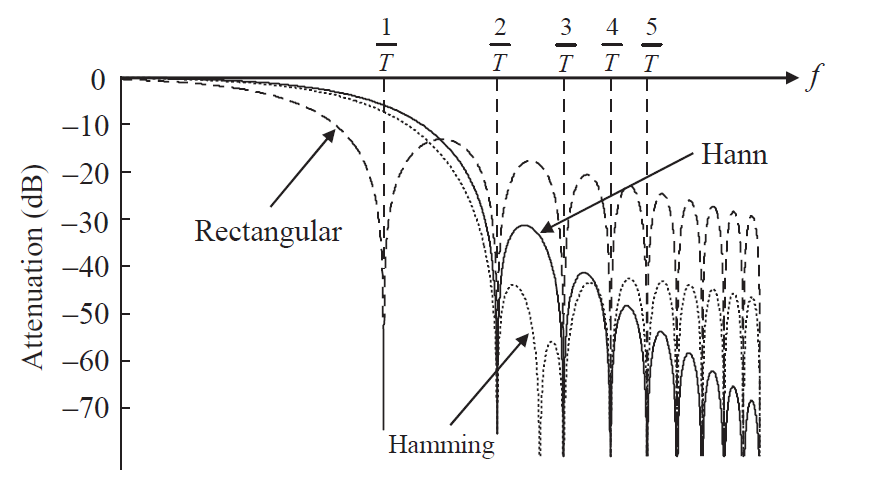
\includegraphics[width=0.8\textwidth]{RespFreqJanelas_ShinHammond.png}
		\caption{Resposta em frequência para três janelas comuns: retangular, Hann, e Hamming (retirado de Shin \& Hammond, 2008).}
		\label{fig:RespFreqJanelas_ShinHammond}
	\end{figure}
	
	Uma das janelas mais populares em Processamento Digital de Sinais é a janela \textbf{Hann} (ou von Hann), definida como:
	
	\begin{equation}
		w[n] = \frac{1}{2}\left[1 - \cos\!\left(\frac{2\pi n}{N-1}\right)\right], \quad n = 0, 1, \ldots, N-1.
		\label{eq:hanning}
	\end{equation}
	
	\subsection{\textit{Zero-Padding}}
	
	O preenchimento com zeros, ou \textit{zero-padding}, consiste em acrescentar zeros ao final do vetor $x[n]$ antes de calcular a DFT, aumentando o comprimento efetivo da transformada de $N$ para $N_{zp} \gg N$:
	
	\begin{equation}
		x_{zp}[n] = \begin{cases} x[n], & 0 \leq n \leq N-1 \\ 0, & N \leq n \leq N_{zp}-1. \end{cases}
	\end{equation}
	
	O zero-padding resulta em uma \textbf{interpolação} no domínio da frequência: o intervalo entre frequências passa a ser $\Delta f_{zp} = f_s / N_{zp}$, fornecendo mais pontos entre as frequências discretas originais $f_k$. Contudo, é importante entender que o \textit{zero-padding} \emph{não aumenta a resolução espectral}: isto é, a capacidade de distinguir duas frequências próximas depende exclusivamente da duração original do registro, $T = N / f_s$.
	
	O \textit{zero-padding} com $N_{zp} \to \infty$ aproxima a \textbf{Transformada de Fourier de Tempo Discreto (DTFT)}, tornando a sequência discreta em uma curva contínua e revelando a ``forma'' do espectro mais claramente. Essa característica o torna útil para visualizações, por exemplo.
	
	% -----------------------------------------------------------------------
	\section{Configuração Inicial}	

	Inicie o seu script Python com as seguintes declarações iniciais:
	
	\begin{lstlisting}[caption={Configurações iniciais comuns a todos os exercícios.}]
import numpy as np
import matplotlib.pyplot as plt

# Parametros do sinal
A  = 2          # amplitude
f0 = 1          # frequencia fundamental [Hz]
Tp = 1./f0      # periodo fundamental [s]
fs = 10./Tp     # frequencia de amostragem (10 amostras por periodo)
dt = 1./fs      # resolucao temporal [s]
	\end{lstlisting}
	
	% -----------------------------------------------------------------------
	\section{Exercícios}
	
	% -----------------------------------------------------------------------
	\subsection*{Exercício 1 — DFT com número inteiro de períodos}
	
	Considere o sinal $x(t) = A\cos(2\pi f_0 t)$, com os parâmetros definidos na Seção 3.
	
	\begin{enumerate}
		\item Gere duas versões do sinal: \texttt{x1} com duração $T_1 = T_p$ (10 amostras) e \texttt{x2} com duração $T_2 = 5 \cdot T_p$ (50 amostras).
		
		\item Para cada sinal, plote seus valores no domínio do tempo. Para evidenciar a hipótese de periodicidade da DFT, inclua também duas repetições periódicas adjacentes a cada lado do sinal.
		
		\item Calcule a DFT de cada sinal usando \texttt{numpy.fft.fft} e plote o espectro de magnitude normalizado $|X[k]|/N$ em função da frequência em Hz.
		
		\item Aplique o \textit{zero-padding} a ambos os sinais, estendendo-os para $N_{zp} = 5000$ pontos. Plote os sinais no domínio do tempo com \textit{zero-padding}, novamente incluindo duas repetições períodicas adjacentes. Em seguida, plote o espectro de magnitude das DFTs com e sem \textit{zero-padding} no mesmo gráfico.
	\end{enumerate}
	
	\textbf{Questões para reflexão:}
	\begin{itemize}
		\item O que você observa no espectro, dado a janela contém um número inteiro de períodos? Onde a energia está concentrada?
		\item O que o \textit{zero-padding} acrescenta ao espectro nesse caso? Ele altera os picos de amplitude?
		\item Como a resolução espectral $\Delta f = f_s/N$ se altera entre \texttt{x1} e \texttt{x2}?
	\end{itemize}
	
	
	% -----------------------------------------------------------------------
	\subsection*{Exercício 2 — Vazamento espectral}
	
	\textcolor{red}{$\rightarrow$ CONTINUAR AQUI!}\\
	Repita o Exercício 1, mas agora com janelas de duração \emph{não inteira} em relação ao período $T_p$:
	
	\begin{itemize}
		\item $T_1 = 1,5 \cdot T_p$ (15 amostras)
		\item $T_2 = 3,5 \cdot T_p$ (35 amostras)
	\end{itemize}
	
	\begin{enumerate}
		\item Plote as formas de onda com suas repetições periódicas e identifique visualmente as descontinuidades nas junções.
		
		\item Calcule e plote os espectros de magnitude (escalonados) com e sem \textit{zero-padding}.
		
		\item Plote também os espectros em escala logarítmica (dB), usando $20\log_{10}(|X[k]|/N)$, com limite inferior de $-60\,\text{dB}$.
	\end{enumerate}
	
	\textbf{Questões para reflexão:}
	\begin{itemize}
		\item Compare com os resultados do Exercício~1. O que muda no espectro quando há descontinuidade na junção periódica?
		\item O vazamento é mais visível em escala linear ou logarítmica? Por quê?
		\item O \textit{zero-padding} consegue eliminar o vazamento espectral? Justifique.
	\end{itemize}
	
	
	% -----------------------------------------------------------------------
	\subsection*{Exercício 3 — Resolução espectral: separando dois componentes}
	
	Considere agora um sinal composto por dois cossenos:
	
	\begin{equation}
		x(t) = A\cos(2\pi f_0 t) + A_b \cos(2\pi f_{0b} t),
		\label{eq:dois_cossenos}
	\end{equation}
	
	com $f_{0b} = f_0 \cdot 2\sqrt{2}$ e $A_b = A/20$ ($\approx -26\,\text{dB}$ abaixo de $A$).
	
	Gere duas versões do sinal:
	\begin{itemize}
		\item \texttt{x1}: duração $T_1 = 2{,}5\,T_p$ (25 amostras) e amplitudes $(A,\, A_b)$
		\item \texttt{x2}: duração $T_2 = 5{,}5\,T_p$ (55 amostras) e amplitudes $(A,\, A/10)$
	\end{itemize}
	
	\begin{enumerate}
		\item Plote as formas de onda com repetições periódicas (sem janelamento, janela retangular implícita).
		
		\item Calcule os espectros com e sem \textit{zero-padding} e plote-os em escala linear e em dB.
		
		\item Identifique nos gráficos a posição esperada de $f_0$ e de $f_{0b}$. O componente de menor amplitude é visível?
	\end{enumerate}
	
	\textbf{Questões para reflexão:}
	\begin{itemize}
		\item Por que o componente $A_b$ não aparece claramente no espectro, apesar de estar presente no sinal?
		\item O que acontece com o componente de menor amplitude à medida que aumentamos $N$? A resolução espectral melhora?
		\item Qual é a influência do nível dos lóbulos laterais da janela retangular na capacidade de detectar componentes de baixa amplitude?
	\end{itemize}
	

	% -----------------------------------------------------------------------
	\subsection*{Exercício 4 — Janelamento para separação espectral}
	
	Repita o Exercício 3, mas agora \textbf{aplique a janela de Hanning} antes de calcular a DFT. No Python, use:
	
	\begin{lstlisting}[caption={Aplicação da janela de Hanning.}]
win1 = np.hanning(N1)
x1_janelado = x1 * win1
	\end{lstlisting}
	
	\begin{enumerate}
		\item Plote as formas de onda janeladas com as repetições periódicas. Sobreponha a curva da janela $A \cdot w[n]$ ao gráfico do sinal. Observe como a janela suaviza as bordas.
		
		\item Calcule os espectros com e sem \textit{zero-padding} e plote-os em escala linear e em dB.
		
		\item Compare os espectros \emph{sem} janela (Exercício~3) e \emph{com} janela de Hanning (este exercício) em escala logarítmica. O componente de menor amplitude se torna visível?
	\end{enumerate}
	
	\textbf{Questões para reflexão:}
	\begin{itemize}
		\item Qual é o compromisso entre redução do vazamento e resolução espectral ao se utilizar a janela de Hanning?
		\item Como o nível dos lóbulos laterais se compara entre a janela retangular e a de Hanning?
		\item Em qual situação prática você escolheria a janela de Hanning em detrimento da janela retangular?
		\item O \textit{zero-padding} aplicado ao sinal janelado ainda produz uma boa aproximação da DTFT? Compare com o caso sem janelamento.
	\end{itemize}
	
	
	% -----------------------------------------------------------------------
	\section*{Referências}
	
	\begin{enumerate}
		\item K.~Shin e J.~Hammond, \textit{Fundamentals of Signal Processing for Sound and Vibration Engineers}. John Wiley and Sons, 2008.
		\item A.~V.~Oppenheim e R.~W.~Schafer, \textit{Discrete-Time Signal Processing}, 3ª~ed. Prentice Hall, 2010.
	\end{enumerate}
	
	\end{document}
	
	
	
\end{document}
